\documentclass[14pt,a4paper,report]{report}
\usepackage[a4paper, mag=1000, left=2.5cm, right=1cm, top=2cm, bottom=2cm, headsep=0.7cm, footskip=1cm]{geometry}
\usepackage[utf8]{inputenc}
\usepackage[english,russian]{babel}
\usepackage{indentfirst}
\usepackage[dvipsnames]{xcolor}
\usepackage[colorlinks]{hyperref}
\usepackage{listings} 
\usepackage{fancyhdr}
\usepackage{caption}
\usepackage{amsmath}
\usepackage{latexsym}
\usepackage{graphicx}
\usepackage{array}
\hypersetup{
	colorlinks = true,
	linkcolor  = black
}

\usepackage{titlesec}
\titleformat{\chapter}
{\Large\bfseries} % format
{}                % label
{0pt}             % sep
{\huge}           % before-code


\DeclareCaptionFont{white}{\color{white}} 

% Listing description
\usepackage{listings} 
\DeclareCaptionFormat{listing}{\colorbox{gray}{\parbox{\textwidth}{#1#2#3}}}
\captionsetup[lstlisting]{format=listing,labelfont=white,textfont=white}
\lstset{ 
	% Listing settings
	inputencoding = utf8,			
	extendedchars = \true, 
	keepspaces = true, 			  	 % Поддержка кириллицы и пробелов в комментариях
	language = C,            	 	 % Язык программирования (для подсветки)
	basicstyle = \small\sffamily, 	 % Размер и начертание шрифта для подсветки кода
	numbers = left,               	 % Где поставить нумерацию строк (слева\справа)
	numberstyle = \tiny,          	 % Размер шрифта для номеров строк
	stepnumber = 1,               	 % Размер шага между двумя номерами строк
	numbersep = 5pt,              	 % Как далеко отстоят номера строк от подсвечиваемого кода
	backgroundcolor = \color{white}, % Цвет фона подсветки - используем \usepackage{color}
	showspaces = false,           	 % Показывать или нет пробелы специальными отступами
	showstringspaces = false,    	 % Показывать или нет пробелы в строках
	showtabs = false,           	 % Показывать или нет табуляцию в строках
	frame = single,              	 % Рисовать рамку вокруг кода
	tabsize = 2,                  	 % Размер табуляции по умолчанию равен 2 пробелам
	captionpos = t,             	 % Позиция заголовка вверху [t] или внизу [b] 
	breaklines = true,           	 % Автоматически переносить строки (да\нет)
	breakatwhitespace = false,   	 % Переносить строки только если есть пробел
	escapeinside = {\%*}{*)}      	 % Если нужно добавить комментарии в коде
}

\begin{document}

\chapter{Домашнее задание №6}

\subsubsection{Бояркин 43501/3}

\section{Применение критерия Найквиста к логарифмическим частотным характеристикам}

Логарифмическая амплитудно-частотная характеристика разомкнутой САР вычисляется по формуле:

\begin{center}
$L(\omega)=20lg|A(\omega|)-20lg|W(j\omega)|$
\end{center}

Логарифмическая фазо-частотная характеристика по формуле:

\begin{center}
$\phi(\omega)=arg(W(j\omega))$
\end{center}

Из частотной характеристики следует, что достижению частотной характеристики окружности единичного радиуса с центром в начале координат при определенной частоте $\omega_c$, называемой \emph{частотой среза} или \emph{граничной частотой}, соответствует пересечение ЛАЧХ $L(\omega)$ оси частот ($L(\omega_c)=0$).

Переходу годографа через вещественную ось при $Re[W(j\omega)]<0$ соответствует переход ЛАФЧХ $\phi(\omega)$ через отметку - $\pi$ (в более сложных случаях, когда частотная характеристика имеет вид спирали - через отметки $\pm \pi, \pm 3\pi, \pm 5\pi, ...$). При этом положительному переходу сооответствует переход ЛФЧХ снизу вверх, а отрицательному переходу - сверху вниз.

Поэтому на основании критерия Найквиста может быть сформулирован \emph{логарифмический частотный критерий устойчивости}.

\section{Логарифмический частотный критерий устойчивости}

Для устойчивости замкнутой САР необходимо и достаточно, чтобы разность между числом положительных и отрицательных переходов ЛФЧХ разомкнутой САР через линию $\pm (2k+1)\pi$ (где $k=0,1,2,...$) при частотах, кгда $L(\omega)>0$, была равна $m/2$.

\begin{figure}[h!]
	\centering
	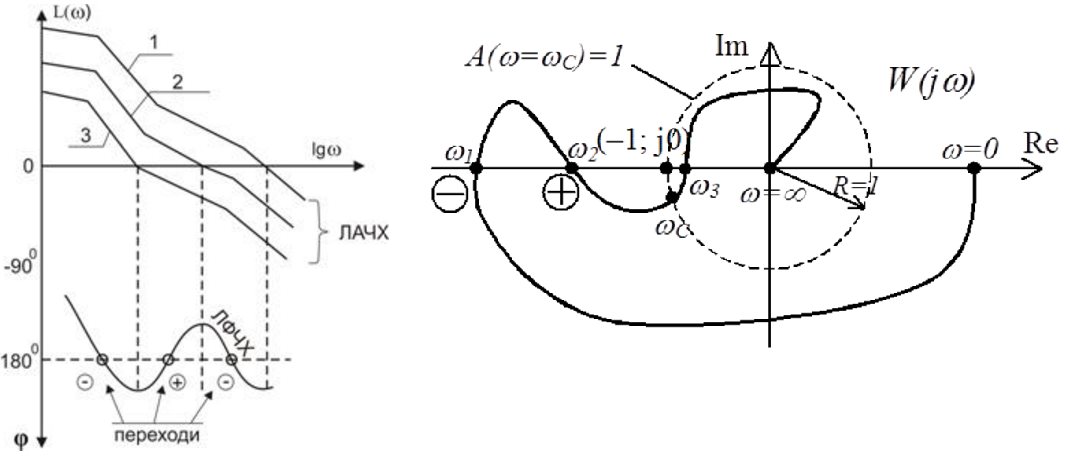
\includegraphics[scale = 0.62]{images/1.png}
	
	\caption{}
	\label{image:20}
\end{figure}





\end{document}